\section{Metriken}
	Zur Analyse von \eeppi\ haben wir drei verschiedene Arten von Metriken erstellt.
	Die erste zeigt den Umfang des Projekts,
	die zweite wie gut wir getestet haben
	und die dritte gibt Auskunft über die Code Qualität.
	
	Auf dem Client wurde mit TypeScript entwickelt, dieses wurde zu JavaScript kompiliert.
	Die Metriken über den Code Umfang wurden für den Clientteil mit den TypeScript-Dateien durchgeführt,
	die restlichen Metriken aufgrund der mangelnden Verfügbarkeit an Tools für TypeScript direkt mit dem JavaScript.
	Dies hat soweit einen Einfluss, dass die Qualität des von TypeScript erzeugten Codes die Messung beeinflusst.
	
	\subsection{Umfang}
	Total setzt sich \eeppi\ aus gut 25'000 Zeilen Code zusammen, inklusive Leerzeilen, Kommentaren, Konfigurationsdaten und Code von anderen Entwicklern.
	Die Zusammensetzung ist in Abbildung\ \ref{fig:TotalSLOC} zu sehen.
	\begin{figure}[H]
		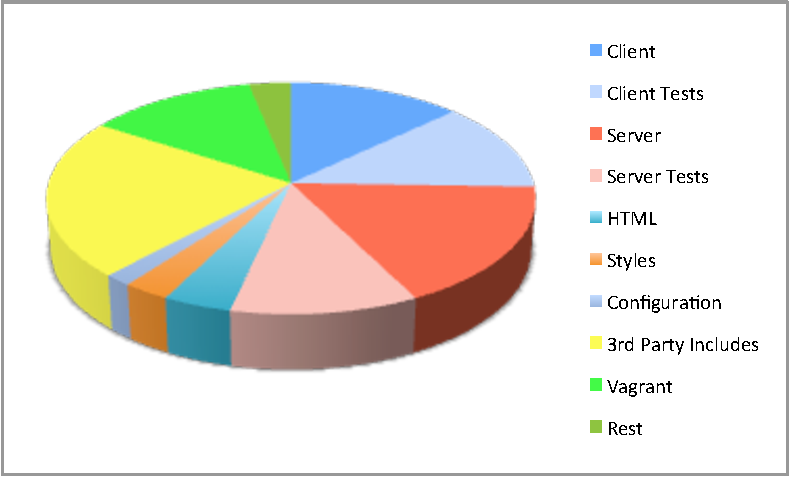
\includegraphics[width=\largeThird\textwidth]{projectPlan/media/img/totalSLOC.pdf}
		\centering
		\caption{Total SLOC (Source Lines of Code)}
		\label{fig:TotalSLOC}
	\end{figure}
	
	Gut die Hälfte des Umfangs entfällt dabei auf unsern Client- und Servercode und seine Tests.
	Ein weiterer grosser Anteil stellen die externen Libraries und Frameworks (22\%),
	sowie die Daten für die Initialkonfiguration der Vagrant-Umgebungen.
	Die restlichen 12\% des Projektes setzen sich zusammen aus Konfiguration, Templates für die Benutzeroberfläche und Styles.
	
	Wird der Hauptteil von \eeppi\ betrachtet (effektiver ausführbarer Code Server- und Client),
	ist zu sehen, dass die Server- und Client in der gleichen Grössendimension liegen.
	Dies war zu erwarten, da sie auch den gleichen Umfang der Daten verarbeiten.
	
	Auch die Tests liegen in der gleichen Grössenordnung.
	Allerdings sind im Client Test Code viele Zeilen an Initialisierungsdaten enthalten zum Mocken\footnote{Das verwendete Test-Framework Angular Jasmine erlaubt das simulieren (mocken) der REST Schnittstelle} der Schnittstellenaufrufe. 
	Die effektive Grösse der Client Tests liegt ca. 25\% tiefer.
	
	Die detaillierte Aufteilung und genaue Anzahl der SLOC (Source Lines of Code) der eigenen Codeteile ist in Abbildung\ \ref{fig:serverClientSLOC} zu sehen.
	
	\begin{figure}[H]
		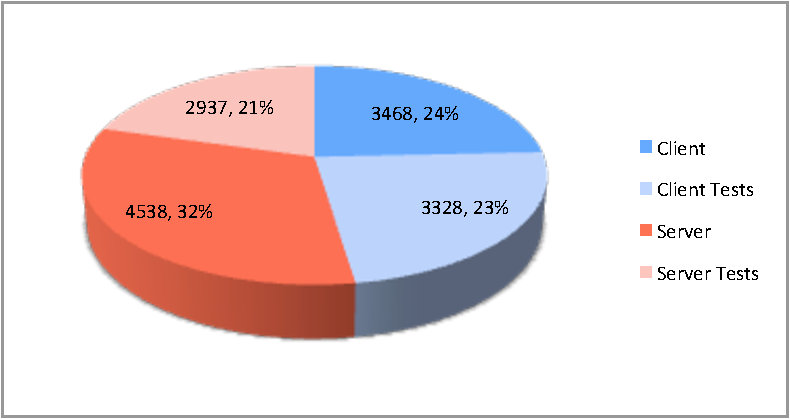
\includegraphics[width=\largeThird\textwidth]{projectPlan/media/img/serverClientSLOC.pdf}
		\centering
		\caption{Vergleich SLOC (Source Lines of Code) auf Server und Client inklusive Tests}
		\label{fig:serverClientSLOC}
	\end{figure}


	\subsection{Test Coverage}
	Sowohl auf dem Server als auch auf dem Client sind wir mehrheitlich nach TDD (Test Driven Development) vorgegangen,
	dementsprechend hoch ist die Testabdeckung.
	Ziel war von Anfang an nicht 100\% Testabdeckung zu erreichen, sondern die wichtigsten Funktionen zu testen.
	
	\begin{figure}[H]
		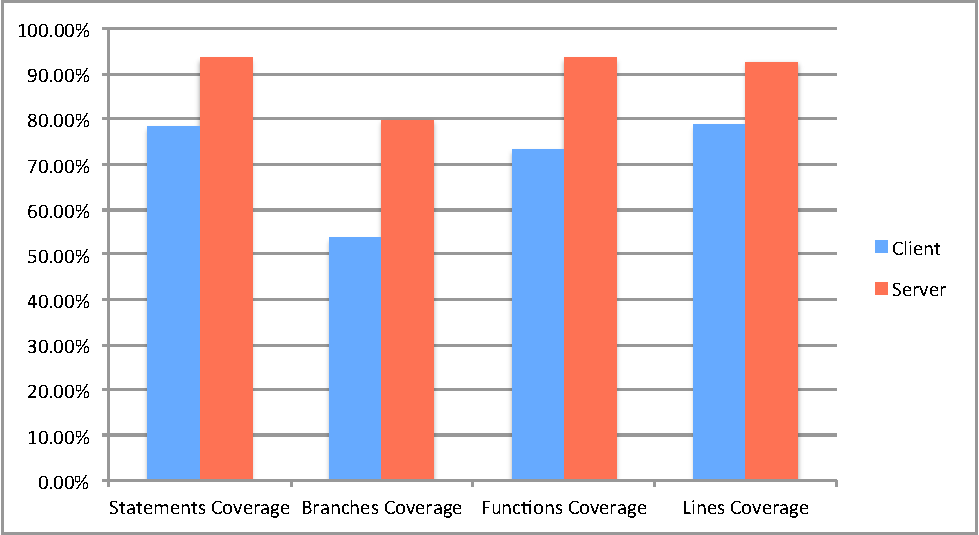
\includegraphics[width=\textwidth]{projectPlan/media/img/coverage.pdf}
		\centering
		\caption{Testabdeckung auf dem Server und dem Client}
		\label{fig:coverage}
	\end{figure}
	
	Abbildung\ \ref{fig:coverage} zeigt die Testabdeckung auf.
	Es ist zu sehen, dass auf dem Server die Testabdeckung höher ist als auf dem Client,
	aber auch auf dem Client sind die zentralen und wichtigen Elemente gut abgedeckt.
	
	
	\subsection{Qualität}
	Die Codequalität ohne grosse Verfälschung zu messen ist eine grosse Herausforderung.
	Hier zeigt sich der erwähnte Einfluss des generierten JavaScripts besonders stark. TypeScript generiert viele anonyme, direkt ausgeführte Funktionen, die der Kapselung des Codes dienen. 
	Der so erzeugte Code drückt die Metriken in die Höhe. Trotzdem lassen sich einige Aussagen treffen anhand der gemessenen Daten.
	
	Wir haben die wichtigsten Kennzahlen evaluiert,
	so die Anzahl der Logical LOC (Anzahl effektiver Code-Zeilen) pro Methode, die Anzahl der Parameter und die Cyclomatic Complexity\footnote{Komplexitätswert der die Operationen pro Methode repräsentiert \url{http://www.aivosto.com/project/help/pm-complexity.html}}.
	
	\begin{figure}[H]
		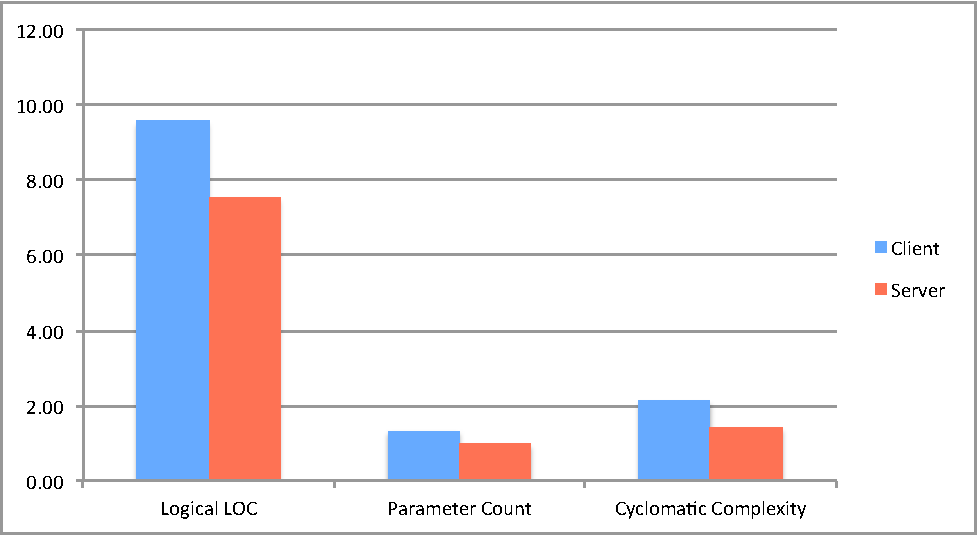
\includegraphics[width=\textwidth]{projectPlan/media/img/methodComplexityOverview.pdf}
		\centering
		\caption{Überblick Durchschnittsmesswerte}
		\label{fig:methodComplexityOverview}
	\end{figure}
	
	In Abbildung\ \ref{fig:methodComplexityLLOC} ist die Anzahl der logischen Zeilen Code pro Methode ausgewiesen.
	Gut sichtbar ist, dass auf dem Server wie auf dem Client rund 35\% aller Methoden drei logische Codezeilen aufweisen.
	Dies sind primär Getter und Setter, bzw. auf dem Client anonyme, von TypeScript erzeugte Methoden.
	
	Zusammengefasst kann man sagen, dass die Mehrheit der Methoden mit weniger als zehn Zeilen Code auskommen und nur einige wenige Methoden mehr Zeilen aufweisen.
	
	\begin{figure}[H]
		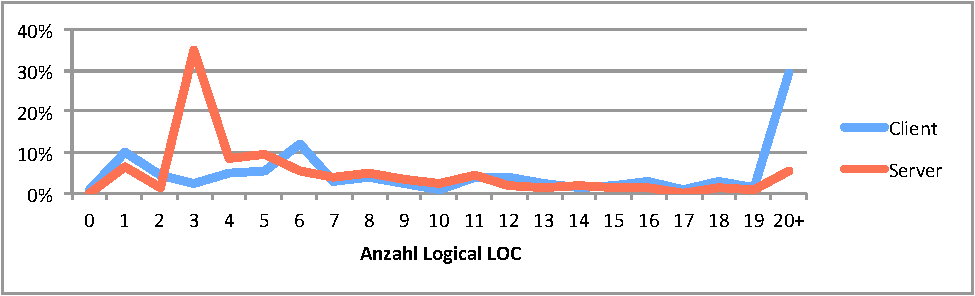
\includegraphics[width=\textwidth]{projectPlan/media/img/methodComplexityLLOC.pdf}
		\centering
		\caption{Anzahl Logical LOC pro Methode}
		\label{fig:methodComplexityLLOC}
	\end{figure}
	
	In Abbildung\ \ref{fig:methodComplexityParameterCount} wird die Häufigkeit der Anzahl Methoden Parameter aufgezeigt.
	Gut erkennbar ist die Tatsache, dass sowohl auf dem Server, wie auch auf dem Client,
	rund 3/4 der Methoden keinen oder nur einen einzigen Parameter besitzen.
	Die Anzahl Methoden mit keinem Parameter ist auf dem Client signifikant tiefer, da aufgrund der Properties in JavaScript das implementieren von Getter für Public-Attributes entfällt.
	
	
	\begin{figure}[H]
		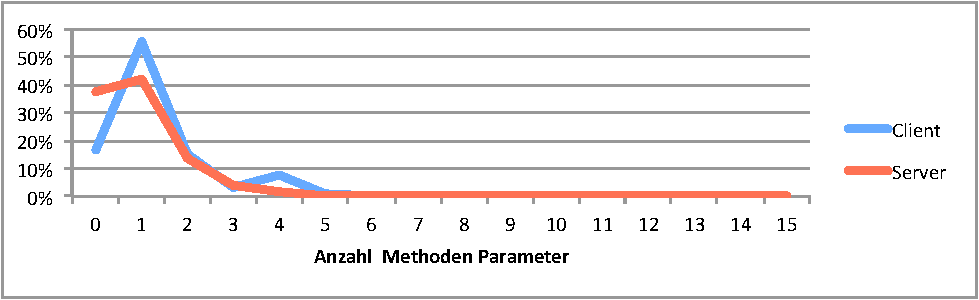
\includegraphics[width=\textwidth]{projectPlan/media/img/methodComplexityParameterCount.pdf}
		\centering
		\caption{Anzahl Parameter pro Methode}
		\label{fig:methodComplexityParameterCount}
	\end{figure}
	Abschliessend ist die Cyclomatic Complexity in Abbildung\ \ref{fig:methodComplexityCyclomaticComplexity} aufgezeichnet.  
	Sie beschreibt, wie viele Operationen eine Methode enthält.
	Die Spitzen bei Eins repräsentieren auch hier die Getter und Setter.
	
	
	\begin{figure}[H]
		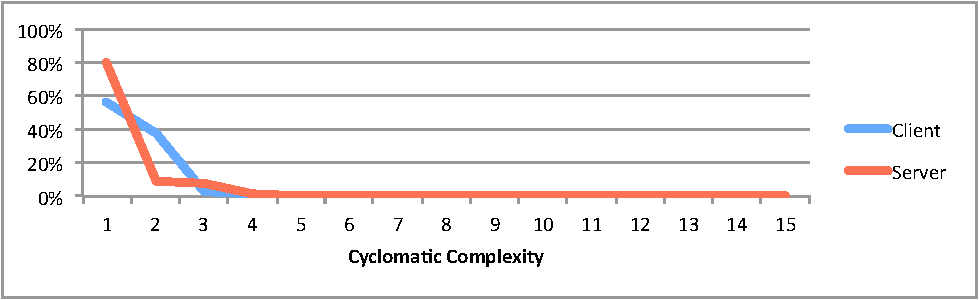
\includegraphics[width=\textwidth]{projectPlan/media/img/methodComplexityCyclomaticComplexity.pdf}
		\centering
		\caption{Cyclomatic Complexity pro Methode}
		\label{fig:methodComplexityCyclomaticComplexity}
	\end{figure}
	
	
	\subsection{Fazit}
		\eeppi\ weist einen ansehnlichen Umfang auf und auch eine gute Testabdeckung.
		Die effektive Höhe  der Codequalität lässt sich jedoch nur schwer eruieren.	
		
		Ungefähr in der Mitte des Projekts hat ein Mitarbeiter des IFS\footnote{Institut für Software, HSR Hochschule für Technik Rapperswil, \url{http://www.ifs.hsr.ch}} einen Codereview durchgeführt und positive Bilanz gezogen.
		Zusätzlich sind aufgrund dieses Feedbacks Verbesserungen in den Code eingeflossen.
		
		Maurice Halstead hat eine Softwaremetrik entworfen,
		welche die Komplexität der Software berechnet und davon ausgehend einige Kennzahlen liefert.
		Eine davon ist die "<Halstead Bugs">, sie gibt die Fehlerkomplexität an,
		also wie viele Fehler die Software aufgrund der berechneten Komplexität und Grösse statistisch ungefähr enthalten könnte.
		Das heisst aber nicht, dass die Software so viele Fehler enthält,
		sondern die Abstraktion mit Bugs ist nur für das bessere Verständnis der Grössenordnung gedacht.
		
		\begin{figure}[H]
			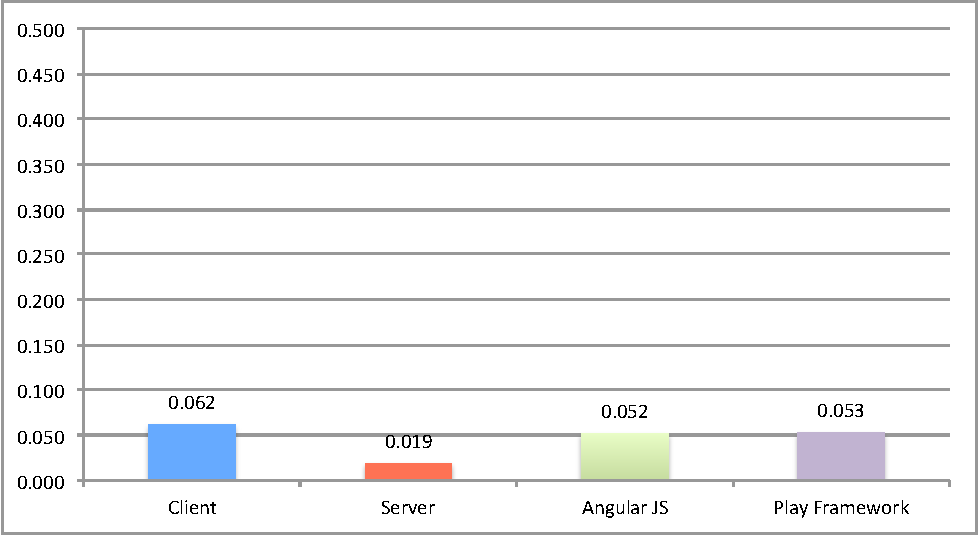
\includegraphics[width=\textwidth]{projectPlan/media/img/halsteadBugsPerMethod.pdf}
			\centering
			\caption{Halstead Bugs pro Methode}
			\label{fig:halsteadBugsPerMethod}
		\end{figure}
		
		In Abbildung\ \ref{fig:halsteadBugsPerMethod} wird diese Komplexitätsgrösse mit zwei der durch \eeppi\ eingesetzten Frameworks verglichen.
		Sowohl der Client als auch der Server weisen einen deutlich besseren Wert aus als die beiden zum Vergleich aufgeführte Frameworks.
		Erstaunlich ist, dass die beiden Frameworks beinahe den gleichen Wert aufweisen.
		
		Beim Anblick der Zahlen liegt die Vermutung nahe, dass es daran liegt,
		dass \eeppi\ einen geringeren Projektumfang hat als die beiden Frameworks.
		Es wird jedoch hier nicht die totale Grösse verglichen, sondern lediglich die Komplexität pro Methode.
		Diese Vermutung trifft deshalb nicht zu.
				
				
	\subsubsection{Typescript}
	Die Ergebnisse werfen auch die Frage auf, was TypeScript bringt und ob es sich dessen Einsatz gelohnt hat.
	
	Aus unserer Sicht hat sich der Einsatz von TypeScript sehr gelohnt. 
	Viele Fehler haben wir dadurch bereits zur Kompilierzeit gefunden und nicht erst zur Laufzeit.
	Der Source Code ist strukturierter, modularisierter, gekapselter und trotzdem lesbarer als vergleichbarer JavaScript Code dies wäre.
	Selbst die Metriken, die anhand des erzeugten JavaScript Codes erstellt wurden, zeigen sehr positive Werte und bestätigten unseren subjektiven Eindruck.	
	
